% Copyright 2020 by Junwei Wang <i.junwei.wang@gmail.com>
%
% This file may be distributed and/or modified under the
% conditions of the LaTeX Project Public License, either version 1.3c
% of this license or (at your option) any later version.
% The latest version of this license is in
%   http://www.latex-project.org/lppl.txt

% \documentclass[aspectratio=169,compress]{beamer}
\documentclass[aspectratio=169,compress]{beamer}

\usepackage[english]{babel}
\usepackage{metalogo}
\usepackage{listings}
\usepackage{fontspec}
\usepackage{tikz}

% \usetheme{Nord}
\usetheme[style=light]{Nord}


%\usepackage[spanish, es-tabla]{babel}
\usepackage[utf8]{inputenc}
\usepackage{hyperref}




\setmainfont{Yanone Kaffeesatz}
%\setsansfont{Andika New Basic}
\setmonofont{DejaVu Sans Mono}

\setbeamerfont{frametitle}{parent=structure,size=\Large}

\AtBeginSection[]
{
  \begin{frame}[c,noframenumbering,plain]
    \tableofcontents[sectionstyle=show/hide,subsectionstyle=show/show/hide]
  \end{frame}
}

\AtBeginSubsection[]
{
  \begin{frame}[c,noframenumbering,plain]
    \tableofcontents[sectionstyle=show/hide,subsectionstyle=show/shaded/hide]
  \end{frame}
}

\title{Arquitecturas y Organización de Computadoras I}
\subtitle{1: Abstracciones en la computadora y tecnología}
\author{Rafael Ignacio Zurita}
\institute{Depto. Ingeniería de Computadoras}
\date{\today}

\begin{document}

\begin{frame}[plain,noframenumbering]
\bigskip
  \maketitle
\end{frame}

% video
% mostrar varias computadoritas
% mostrar placa con integrados y pcb
% mostrar foto de chip y hablar de los transistores
% mostrar imagen wakerly de transistor CMOS

% imagenes 
% foto de performance
% cuadro python vs C
% foto eras tecnologicas

% historia de ibm
% fotos de computadoras hitos
%     ibm 360 (mainframe), cray1 (supercoputaodra)
%     pdp-11 (creacion de unix) (minicomputadora)
%     4004 primer chip integrado
%     apple II y ibm pc (computadora personal)
%     open mobile komunications (smartphones)
%     iphone smartphone

\section{Abstracciones en la computadora y tecnología}

\subsection{Eras tecnológicas}
\subsection{Limitaciones tecnológicas}
\subsection{Tiempo de ejecución (rendimiento)}
\subsection{Terminología: Arquitectura y Organización de un procesador}
\subsection{Avances (cuadro)}
\subsection{MIPS/RISCV ISA (Arquitectura de una computadora real)}

\subsection{Abstracciones en la computadora}

\begin{frame}{La computadora: Un sistema complejo}{CHIP}

    \begin{columns}[onlytextwidth,T]
      \column{\dimexpr\linewidth-60mm-5mm}

	\begin{itemize}
	\begin{small}
  \item[Chip] Die en inglés, es empaquetado dentro de un componente que permite su utilizacióin mecánica en un PCB.

\bigskip
\item[Densidad] La tecnología que se utiliza para fabricar los chips (dies), en los circuitos integrados, es el trasistor CMOS.\\
Actualmente la densidad es tan grande que existen miles de millones de transistores en un unico chip.

	\end{small}
	\end{itemize}

      \column{60mm}
    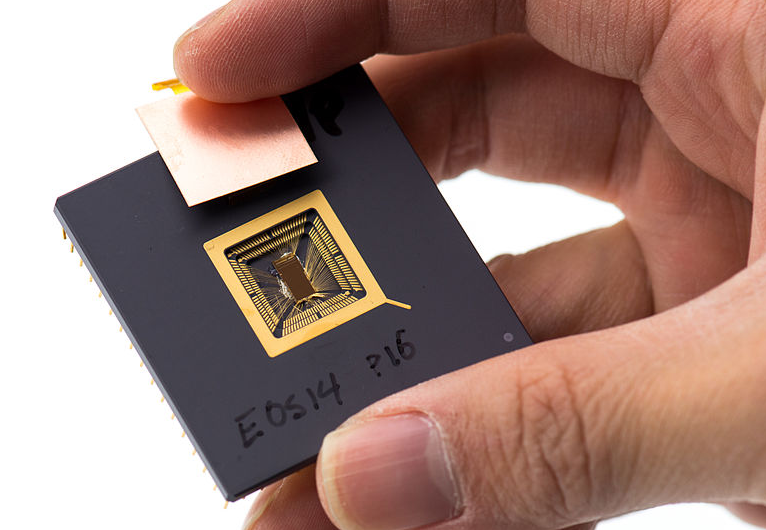
\includegraphics[width=50mm]{images/chip.png}

    \end{columns}

\begin{frame}{La computadora: Un sistema complejo}

    \begin{columns}[onlytextwidth,T]
      \column{\dimexpr\linewidth-60mm-5mm}

	\begin{itemize}
	\begin{small}
  \item[Abstracción] El hardware y software de una computadora
consiste de una jerarquía en capas, donde cada capa de hardware o software
le oculta detalles a la capa superior.

\bigskip

\item[Principio] \textit{El principio de abstracción} es el que \textit{permite}
a los diseñadores de hardware y software poder \textit{entender la complejidad} 
de los sistemas de cómputo que construyen.

\bigskip

\item [Interfaz] EL nivel \textit{Arquitectura del Conjunto de 
Instrucciones (ISA)}, es la interfaz entre el hardware y el software.

	\end{small}
	\end{itemize}

      \column{60mm}
    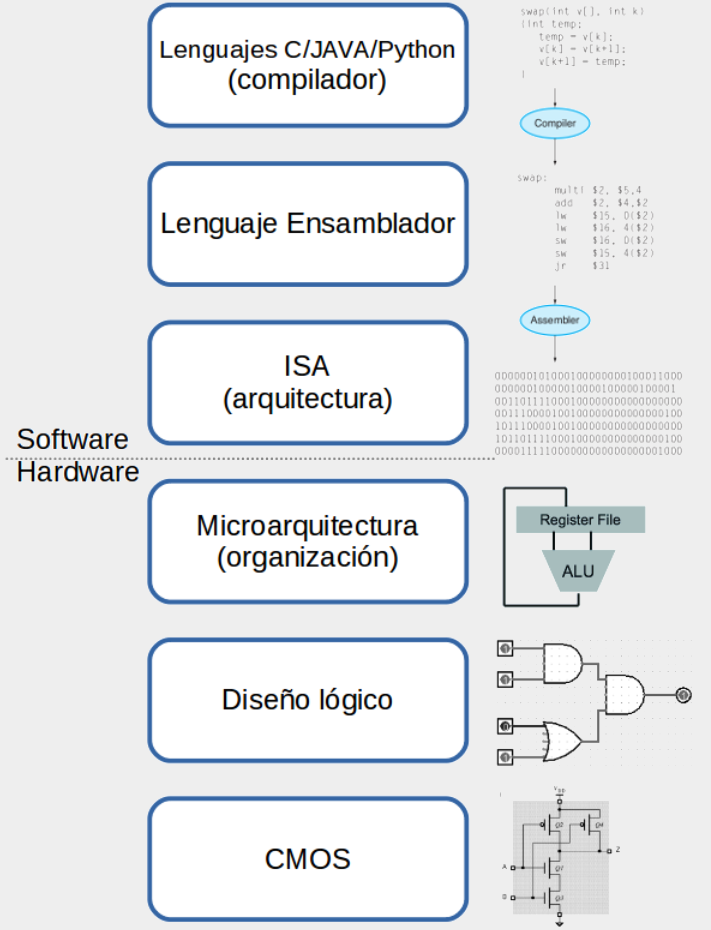
\includegraphics[width=50mm]{images/abstracciones2.png}

    \end{columns}

\end{frame}



%\begin{frame}{La computadora: Un sistema complejo}

%   \begin{columns}[onlytextwidth,T]
%   \column{\dimexpr\linewidth-60mm-5mm}


%  \begin{description}[Snow Storm]
%  \begin{small}
%  \item[Abstracción] El hardware y software de un procesador
%consiste de una jerarquía en capas, donde cada capa le oculta
%detalles a la capa superior.

%\bigskip

%\item[Principio] Este principio de abstracción es el que permite
%a los diseñadores de hardware y software entender la complejidad 
%de las computadoras.

%\bigskip

%\item [Interfaz] EL nivel \textit{Arquitectura del Conjunto de 
%Instrucciones (ISA)}, es la interfaz entre el hardware y el software.

%\end{small}
%  \end{description}

%    \column{60mm}
%    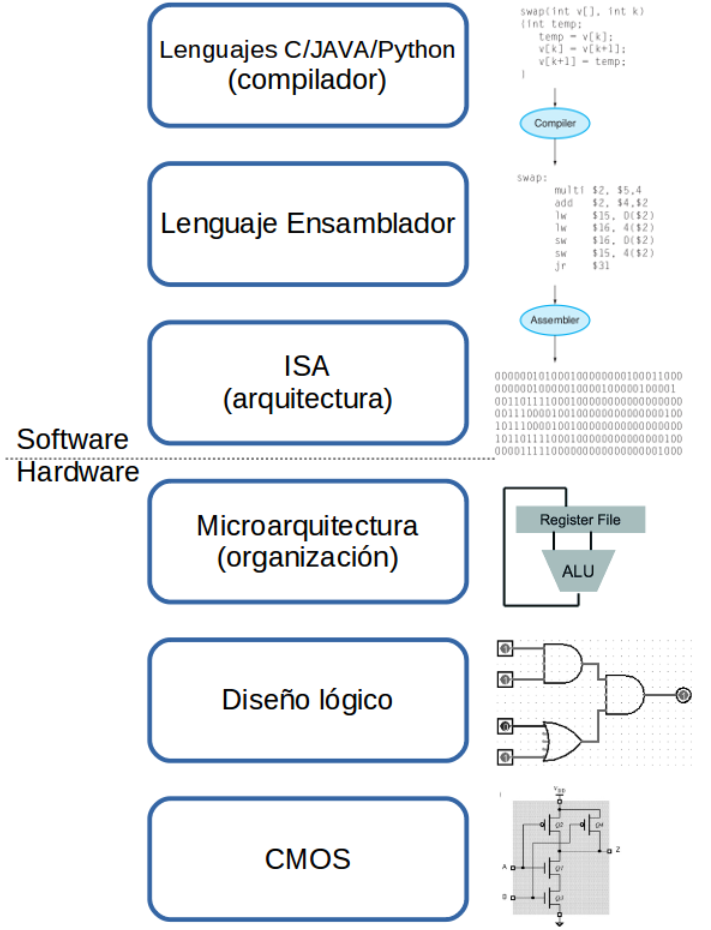
\includegraphics[width=60mm]{images/abstracciones.png}

%    \end{columns}

%\end{frame}


\subsection{Modalidad Virtual}


\begin{frame}[fragile]
  \frametitle{Año 2020 - modalidad virtual}
  Durante la no presencialidad la clase teórica será la siguiente manera:

\bigskip
\begin{itemize}
\item La primer hora se dedicará a revisar el material del día:
\begin{itemize}
\item Video de la clase
\item Apunte de uno de los temas conceptuales
\end{itemize}
\end{itemize}

\bigskip

\begin{itemize}
\item Durante la segunda hora se realizará:
\begin{itemize}
\item Consultas por chat o audio utilizando el canal de telegram
\item Consulta y discuciones del tema del día por meet
\item Exposición espontánea o planificada
\end{itemize}
\end{itemize}

\end{frame}

\begin{frame}[fragile]
  \frametitle{Año 2020 - modalidad virtual}
  Durante la no presencialidad la clase práctica será la siguiente manera:

\bigskip
\begin{itemize}
\item Primera hora: canal de telegram para consultas por audio o chat
\bigskip
\item Segunda hora: participación en clase.
\begin{itemize}
\item Se expondrá de manera oral la resolución de un ejercicio de la práctica.
\item La participación puede ser espontánea.
\item La participación puede ser planificada (la cátedra indica que alumnos deben exponer la resolución).
\end{itemize}
\end{itemize}

\end{frame}

\subsection{¿Por qué (o para qué) se estudia AyOdC?}

\begin{frame}[fragile]
  \frametitle{¿Por qué (o para qué) se estudia AyOdC?}
\begin{small}
\textit{"The next decade will see a Cambrian explosion of novel computer architectures, meaning exciting times for computer architects in academia and in industry."}
John L. Hennessy y David A. Patterson 
(A New Golden Age for Computer Architecture, ACM, 2019)
\end{small}

\bigskip
\begin{small}
\begin{itemize}
\item Grandes empresas (como Google, IBM, Intel, Apple, Cisco,...)
solicitan \\ que los candidatos conozca sobre arquitecturas (ARM/x86/RISCV).\\
(Entendiendo la arquitectura de una computadora puede ayudar a obtener empleo).

\item Los ingenieros de software con mas experiencia entienden \\ como funciona el hardware debajo de sus programas.

\item Para estudiar conceptos en capas abstractas superiores: \\
En las materias relativas a lenguajes de programación, sistemas operativos, y programación de sistemas embebidos se requiere conocer arquitecturas de computadoras.

\end{itemize}
\end{small}

\end{frame}




\begin{frame}[fragile]
  \frametitle{¿Por qué (o para qué) se estudia AyOdC?}

\begin{small}
\begin{itemize}
\item Los empleos para ingenieros de software suelen \\ contar 
con muchos candidatos (programadores de python/java/go/ruby).

\item Los sistemas embebidos son el futuro:
\begin{itemize}
\item Redes de sensores
\item Reproductores multimedia
\item Smartphones
\item Smart TVs
\item Radares
\item Satélites
\item Cualquier aparato conectado a internet (iot)
\end{itemize}

\item Entender la arquitectura de una computadora es clave \\ para programar un sistema embebido.

\end{itemize}
\end{small}

\end{frame}




\subsection{No todas son ventajas...}

\begin{frame}[fragile]
  \frametitle{No todas son ventajas...}

\begin{small}
\begin{itemize}

\item El hardware no suele ser amigable

\begin{itemize}
\item Muchísimos detalles de bajo nivel.
\item A veces es contradictorio.
\end{itemize}

\item El hardware es complejo
\begin{itemize}
\item  El reloj es importante
\item Un pequeño agregado en la funcionalidad puede \\
requerir modificaciones o agregados a muchas piezas de hardware.
\end{itemize}
\item La temática es tan extensa que no es posible \\
cubrirlo en una materia.
\item Es necesario analizar temas de formas nuevas.

\end{itemize}
\end{small}

\end{frame}


\subsection{Recursos}

\begin{frame}[fragile]
  \frametitle{Recursos de la materia}

\begin{small}
\begin{itemize}

\item Web: \footnotesize{\texttt http://se.fi.uncoma.edu.ar/ayod1c/}\\
(se alcanza también desde la materia en PEDCO).

\item FOROs de PEDCO (Novedades y Consultas)
\item Telegram (para consultas)
\item Google meet para las exposiciones y discuciones temáticas online\\ (se darán los enlaces de encuentros en las clases).
\item Bibliografía:

\begin{itemize}

\item Andrew S. Tanenbaum (2000), ORGANIZACIÓN DE COMPUTADORAS un enfoque estructurado, Editorial Prentice Hall. (10 copias en biblioteca)
\item David. Patterson, John L. Hennessy, ORGANIZACIÓN Y DISEÑO DE COMPUTADORES La interfaz hardware/software, McGraw-Hill (8 copias en biblioteca).
\item Apuntes y artículos en la web de la materia
\item David. Patterson, John L. Hennessy, Computer Organization and Design RISC-V Edition 1st Edition The Hardware Software Interface. ISBN: 9780128122754

\end{itemize}

\end{itemize}
\end{small}

\end{frame}


\end{document}

%%% Local Variables:
%%% mode: latex
%%% TeX-master: t
%%% TeX-engine: xetex
%%% End:
